\documentclass{easychair}

% \usepackage{doc}
\usepackage{setspace}
\usepackage{verbatim}
\usepackage{amssymb}
\usepackage[straightquotes]{newtxtt}

%----Suppress extra space in texttt mode
\AddToHook{cmd/ttfamily/after}{\frenchspacing}

%----Making things more compact
\newcommand{\smalltt}[1]{\small \texttt{#1}}
\newenvironment{packed_itemize}{
\vspace*{-0.3em}
\begin{itemize}
\setlength{\partopsep}{0pt}
\setlength{\itemsep}{1pt}
\setlength{\parskip}{0pt}
\setlength{\parsep}{0pt}
}{\end{itemize}}
\newenvironment{packed_enumerate}{
\vspace*{-0.3em}
\begin{enumerate}
\setlength{\partopsep}{0pt}
\setlength{\itemsep}{1pt}
\setlength{\parskip}{0pt}
\setlength{\parsep}{0pt}
}{\end{enumerate}}
% \renewcommand{\textfraction}{0.07}
% \renewcommand{\topfraction}{0.9}
% \renewcommand{\bottomfraction}{0.9}
% \renewcommand{\floatpagefraction}{0.66}
% \setlength{\floatsep}{2.0pt plus 2.0pt minus 2.0pt}
% \setlength{\textfloatsep}{5.0pt plus 2.0pt minus 0.0pt}

\title{The New TPTP Format for Interpretations}

\author{
  Geoff Sutcliffe\inst{1}
\and
  Alexander Steen\inst{2}
\and
  Pascal Fontaine\inst{3}
}

\institute{
  University of Miami,
  Miami, USA\\
  \email{geoff@cs.miami.edu,jam771@miami.edu}
\and
  University of Greifswald,
  Greifswald, Germany\\
  \email{alexander.steen@uni-greifswald.de}
\and
  University of Li{\`e}ge,
  Li{\`e}ge, Belgium\\
  \email{Pascal.Fontaine@uliege.be}
}

\authorrunning{Sutcliffe, Steen, Fontaine}
\titlerunning{TPTP World Interpretations}

\begin{document}
\maketitle

%--------------------------------------------------------------------------------------------------
\begin{abstract}
This paper describes the new TPTP format for representing interpretations.
It provides a background survey that helped us ensure that the representation format is adequate
for different types of interpretations, including Tarskian, Herbrand, and Kripke interpretations.
The needs of applications that use models output by model finding ATP systems are considered.
The syntax and semantics of the new format is expounded in detail, with multiple examples.
Verification of models is discussed and an implementation is presented.
Some tools that support processing the new format are noted.
The properties of interpretations represented in the new format are discussed.
\end{abstract}
%--------------------------------------------------------------------------------------------------
\section{Introduction}
\label{Introduction}

Historically, Automated Theorem Proving (ATP) has, as the name suggests, focused largely on the
task of proving theorems from axioms -- the derivation of conclusions that follow inevitably 
from known facts \cite{RV01-HAR}.
The axioms and the conjecture to be proved (and hence become a theorem) are written in an 
appropriately expressive logic, and the proofs are often similarly written in logic \cite{SS+06}.
In the last two decades the converse task of disproving conjectures, i.e., proving that a 
conjecture is not a theorem of the axioms, has become increasingly important.
This process depends on finding a {\em countermodel} for the conjecture, i.e., an 
{\em interpretation} (a structure that maps formulae to truth values) that is a {\em model}
of the axioms (maps the axioms to $true$) but not a model for the conjecture (maps the conjecture
to $false$).
A salient application area that uses this form of ATP is verification \cite{DKW08}, where a 
countermodel is used to pinpoint the reason why a proof obligation fails, and correspondingly 
points to the location of the fault in the system being verified.
Other applications of model finding include checking the consistency of an axiomatization 
\cite{SS+17}, and finding a solution to a problem that is coded as a model finding problem 
\cite{Win82}.

The TPTP World \cite{Sut17} (\href{https://www.tptp.org}{\tt www.tptp.org}) is a well established 
infrastructure that supports research, development, and deployment of 
% Automated Theorem Proving 
ATP systems.
Various parts of the TPTP World have been deployed in a range of applications, in both academia 
and industry.
The TPTP World includes the TPTP problem library \cite{Sut09}, 
the TSTP solution library \cite{Sut10}, 
tools and services for processing ATP problems and solutions \cite{Sut10}, 
it supports the CADE ATP System Competition (CASC) \cite{Sut16}.
The TPTP language \cite{Sut23-IGPL} is one of the keys to the success of the TPTP World.
Originally the TPTP World supported only first-order clause normal form (CNF)
\cite{SS98-JAR}.
Over the years full first-order form (FOF)
\cite{Sut09}, 
typed first-order form (TFF)
\cite{SS+12,BP13-TFF1}, 
typed extended first-order form (TXF)
\cite{SK18}, 
typed higher-order form (THF)
\cite{SB10,KSR16}, 
and non-classical forms (NXF, NHF).
Most relevant to this work, the TPTP languages are used for writing ATP problems, 
derivations, and interpretations \cite{SS+06,Sut08-KEAPPA}.
Examples of problems are in Appendices~\ref{FOF_Finite.p}, \ref{TFF_Finite.p},
\ref{TFF_Infinite.p}, \ref{THF_Finite.p}, \ref{NXF_Finite-Finite-Global.p}, 
and~\ref{NXF_Finite-Finite-Local.p}.

A TPTP format for interpretations with finite domains was previously been defined \cite{SS+06},
and has served the ATP community adequately for almost 20 years. 
The old format is output by several ATP systems, e.g., Paradox \cite{CS03}, FMDarwin \cite{BF+06}, 
Vampire \cite{KV13}.
Recently the need for a format for interpretations with infinite domains, and for a format for 
Kripke interpretations \cite{Kri63}, has led to the development of a new TPTP format for 
interpretations.
This work describes the new format.
The underlying principle is unchanged: interpretations are represented in formulae.

\paragraph{Related Work:}
There are other concrete representations of interpretations in use:
The SMT-LIB standard \cite{BFT17} defines a format for model output, and commands to inspect 
models.  
SAT solvers generally output models as specified by the SAT competitions \cite{JL+12}, in a 
simple format similar to the DIMACS input format \cite{Bab93}.
Some individual model finding systems have defined their own formats for models, e.g., the 
output formats of Nitpick and Z3 \cite{dMB08}.
% +++
% Nikolaj says ...
% Z3 It produces models that define functions by expressions. For example a model of succ is 
% Succ(x) =X+ 1
% Works when domain is integer. Currently z3 does not implement infinite models for uninterpreted sorts. I would probably support infinite sorts by creating injection into an algebraic datatype and then support models that can be expressed over ADT.
% See also https://microsoft.github.io/z3guide/docs/logic/Quantifiers
% +++

\vspace*{1em}
This paper is organized as follows:
Section~\ref{Interpretations} discusses the nature of interpretations, considering what is
needed from interpretations, and the various forms that interpretations can take.
Section~\ref{NewTarskian} defines the new format for Tarskian interpretations, and
Section~\ref{NewKripke} does the same for Kripke interpretations.
% Section~\ref{Verification} describes the semantic approach to model verification.
Section~\ref{Conclusion} concludes and discusses plans for future work.

%--------------------------------------------------------------------------------------------------
\section{About Interpretations}
\label{Interpretations}

%--------------------------------------------------------------------------------------------------
\subsection{What do we Need?}
\label{Need}

The needs of applications that use model finding vary according to their use of the model.
In the simplest case application need only to know that a model exists.
Examples of such applications include checking the consistency of an axiomatization \cite{CI15},
use as a subroutine in more complex reasoning, e.g., for
axiom selection \cite{SP07,Pud07-ESARLT}, and establishing the existence of a bug in a
verification process\footnote{%
Bill McCune claimed that establishing the existence of a bug without having an explicit model
to help pinpoint the bug would be ``frustrating''. And he should have known.}.
A key weakness of model finder systems that claim to have found a model but do not output an 
explicit model is that it is necessary to trust the model finder.

In many applications it is necessary to have an explicit model, in some representation format that
allows for analysis of the model.
Applications that productively use an explicit model include finding inconsistencies in 
axiomatizations \cite{SS+17}, identification of bugs in verification \cite{CE82,QS82},
solution of problems encoded as a model finding problems \cite{Win82}, and evaluating formulae
wrt the model \cite{SS+23-LPAR}.
Manual inspection of explicit models can also be useful, e.g., \cite{EK+10}.
Explicit models can be used for machine learning and improving model finders internally.
A key advantage of having an explicit model output is that the model can be verified, i.e., the
model finder does not need to be trusted,

Given the innate desirability of obtaining explicit models of satisfiable formulae, desirable
properties of interpretation representation can be considered.
\begin{packed_itemize}
\item Verification of models (checking that the formulae evaluate to $true$ wrt the model), 
      should be possible.
\item Evaluation of formulae wrt an interpretation should be tractable.
      This correspnds to the {\em atom test} and {\em formula evaluation} postulates suggested
      by \cite{FL96,CLP04}.
\item Interpretations should be sufficiently comprehensible for manual inspection.
\end{packed_itemize}

%--------------------------------------------------------------------------------------------------
\subsection{What do we Have?}
\label{Have}

A {\em Tarskian interpretation} \cite{TV56} of formulae in first-order logic consists of a 
non-empty domain of unequal elements for each type used in the formulae (just one domain for 
untyped logic), and mappings for the function and predicate symbols with respect to the 
domains \cite{Hun96,Gal15}.
An overview of some ways of building and representing Tarskian interpretations is provided 
by \cite{CLP04}, and \cite{Pel03-EQMC} provides a comprehensive list of approaches.
A {\em complete} interpretation can interpret all expressions that can be written in the language 
of the formulae, but a {\em partial} interpretation can interpret only (at least) the 
given formulae, e.g., \cite{BSW23}.
Two types of Tarskian interpretations are clear (and more might exist)~\ldots
\begin{packed_itemize}
\item {\em Finite} Tarskian interpretations have only finite domains.
      The domain and symbol mappings can be be explicitly enumerated.
      Finite models for a set of formulae are typically produced by starting with domains of 
      size one, and incrementing the sizes until a model is found.
      At each iteration the formulae are reduced to either propositional 
      \cite{CS03,McC03-MACE4-TR} or function free \cite{BF+09} logic, both of which are decidable.
      An ATP system can then decide if there is a model.
      There are several ATP systems that produce finite Tarskian models, e.g., Paradox, FMDarwin, 
      and Vampire.
\item {\em Infinite} Tarskian interpretations have one or more infinite domains.
      Infinite domains can be explicitly generated (e.g., terms representing Peano numbers) or 
      implicitly specified (e.g., some set of algebraic numbers, such as the integers) \cite{BB13}.
      % HOW IS THIS DONE?
      There are some ATP systems that produce infinite Tarskian models, e.g., 
      cvc5 \cite{BB+22-cvc5} and Z3.
\end{packed_itemize}
\vspace*{-0.5em}
Formulae can be interpreted wrt (finite) Tarskian interpretations~\ldots
\begin{packed_itemize}
\item Interpret quantifiers using Tarskian semantics.
\item Interpret ground (grounded with domain elements) terms and atoms using the mappings.
\item Interpret boolean formulae using the truth tables for connectives.
\end{packed_itemize}
\vspace*{-0.5em}
This approach is taken internally in Vampire.

\vspace*{0.8em}
A {\em Herbrand interpretation} \cite{Her30} has the Herbrand universe as the domain, the mapping 
for non-boolean symbols (functions) is the ``identity'', and the mapping for boolean symbols 
(predicates) is from the Herbrand base to $\{true,false\}$.
Every set of formulae induces its set of Herbrand models.
Such sets can be the result from an ATP system applying model preserving transformations to its 
input (even the input iteself induces its set of Herbrand models), or be generated by an ATP 
system with the explicit intention of representing Herbrand models:
\begin{packed_itemize}
\item {\em Formulae} that are intended to represent Herbrand interpretations, written 
      {\em Herbrand-formulae} to avoid confusion, can be produced.
      Examples include saturations (discussed separately in the next bullet point), a disjunction 
      of implicit generalisations (DIGs) \cite{LM87}, sets of constrained unit clauses 
      \cite{CZ92,CP95,CP95-TAB}, SGGS clause sequences \cite{BP16}, various representations of 
      tableaux (as long as you use a proof confluent calculus, it is normally possible to construct 
      a model from a saturated branch) \cite{Hah01}, eq-interpretations \cite{Pel03-EQMC}, and 
      predicate definitions over the term algebra \cite{SK12}.
      iProver \cite{Kor08,SK12} is an ATP system that outputs the latter format.
\item {\em Saturations} \cite{BG+01,Pel03-JSC} are a fixed point for a set of clauses at which 
      further application of a complete inference system does not generate any new clauses.
      This approach is adopted in saturation-based ATP systems such as E \cite{SCV19},
      Prover9 \cite{McC-Prover9-URL}, Vampire, and Zipperposition \cite{VB+21}.
\end{packed_itemize}
While the domain of the Herbrand interpretations induced by a saturation is known to be the 
Herbrand Universe, there might not be an explicit symbol interpretation that can be used 
constructively by users.

A {\em Kripke interpretation} \cite{Kri63} adds a layer of {\em worlds} over Tarskian 
interpretations.
There can be a finite or infinite number of worlds.
There is an {\em accessibility relation} between the worlds, which can be subject to the
requirements of the logic being used, e.g., for modal logic {\bf M} the accessibility 
relation must be reflexive.
Within each world there is a Tarskian interpretation, and there can be some interaction
between the worlds' Tarskian interpretations if the terms designate globally MORE TO BE SAID.
Formulae can be interpreted wrt Kripke interpretations (with finite worlds and local terms)~\ldots
\begin{packed_itemize}
\item Interpret quantifiers over worlds using Kripke semantics.
\item Interpret formulae within a world wrt the Tarskian interpretation in the world.
\end{packed_itemize}

The notions of interpretations, models, partial interpretations, finite interpretations,
Herbrand interpretations, etc., are captured in the SZS ontologies \cite{Sut08-KEAPPA}, as
updated at 
\href{https://www.tptp.org/cgi-bin/SeeTPTP?Category=Documents\&File=SZSOntology}{\tt www.tptp.org}
\href{https://www.tptp.org/cgi-bin/SeeTPTP?Category=Documents\&File=SZSOntology}{\tt /cgi-bin/SeeTPTP?Category=Documents\&File=SZSOntology}.
For this work the ontology was extended with a new value {\em Model Preserving} (MPR), defined
as ``Some interpretations are models of Ax, and
  all models of Ax are extended to a model of C, and
  all models of C are an extension of a model of Ax
  (which means that all models of C are models of Ax)''.
This is used for transformations on satisfiable sets of formulae in which the models of the set 
are unchanged, or are changed only by adding new domain elements or mappings, so that the
extended models are still models of the original set of formulae. 
Examples of such transformations are adding logical consequence of the set into the set, and
Skolemization.

%--------------------------------------------------------------------------------------------------
\subsection{Do we Have what we Need?}
\label{HaveNeed}

The new TPTP format for interpretations represents Tarskian and Herbrand interpretations in 
{\em interpretation-formulae} -- the details are provided in Sections~\ref{NewTarskian} 
and~\ref{NewKripke}.
Interpretation-formulae are written in an extension of the language of the formulae being 
interpreted, i.e., extending the vocabulary but still using TPTP syntax.

Figure~\ref{ModelLandscape} provides an overview of the situation.
The starting point is the set of {\sf Satisfiable formulae in $\Sigma$}, which might have been
formed from {\sf Ax $\cup$ \{{\raisebox{0.4ex}{\texttildelow}}C\}}. 
$\Sigma$ is the language of the formulae.
Going down leads to the {\sf Models} of the satisfiable formulae.
Some of the models are Tarskian models, and some are Herbrand models.
Going left from the {\sf Satisfiable formulae in $\Sigma$} is the pathway taken by ATP systems 
that find a Tarskian model, and output interpretation-formulae representing the model.
If the interpretation-formulae correctly represents a model of the satisfiable formulae, then
the satisfiable formulae can be proved ($\vDash$) from the interpretation-formulae.
The models of the interpretation-formulae are a subset ($\subseteq$) of the models of the
satisfiable formulae.
Going right from the {\sf Satisfiable formulae in $\Sigma$} is the pathway taken by ATP systems
that apply model preserving transformations ({\sf MPR}s) on the satisfiable set, possibly 
including conversion to CNF with Skolemization, to produce formulae that induce a set of 
Herbrand models of the original {\sf Satisfiable formulae in $\Sigma$}.
The {\sf Satisfiable formulae in $\Sigma$} can be proved from the sets that result from applying 
MPRs

\begin{figure}[htbp]
\centering
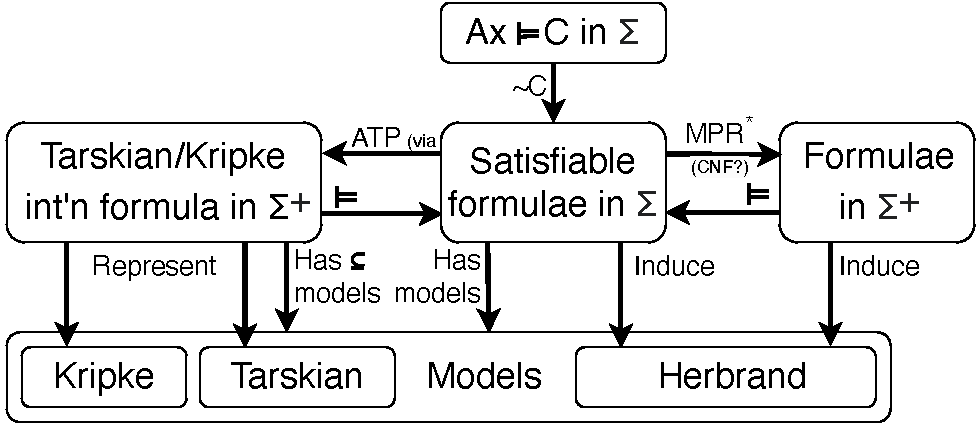
\includegraphics[width=0.75\textwidth]{ModelLandscape.pdf}
\caption{A Landscape of Classical Logic Model Building}
\label{ModelLandscape}
\end{figure}

To interpret a formula wrt interpretation-formulae~\ldots
% $\varphi$ wrt a given interpretation $I$ ($I\,\vdash\,\Phi$ means that 
% $\Phi$ is $true$ in $I$, i.e., $I$ is a model of formula $\Phi$)~\ldots
\begin{packed_itemize}
\item For Kripke interpretation-formulae, theorem proving can be used.
      This is described in Section~\ref{KripkeVerification}.
\item For Tarskian interpretation-formulae, theorem proving can be used.
      \begin{packed_itemize}
      \item If a formula can be proved from the interpretation-formulae then it is $true$ in the 
            interpretation represented by the interpretation-formulae.
      \item If a formula can be disproved from the interpretation-formulae then it is $false$ in 
            the interpretation represented by the interpretation-formulae.
      \item In practice, a formula might be neither proved nor disproved within reasonable 
            resource limits, so that nothing is known.
      \end{packed_itemize}
\item For Herbrand interpretations induced by saturations or Herbrand-formulae, theorem proving 
      can be used~\ldots
      \begin{packed_itemize}
      \item If a formula can be proved from the saturation or Herbrand-formulae then it is 
            $true$ in all the Herbrand interpretations induced by the saturation or 
            Herbrand-formulae.
      \item If a formula can be disproved from the saturation or Herbrand-formulae then it is 
            $false$ in in all the Herbrand interpretations induced by the saturation or 
            Herbrand-formulae.
      \item In practice, a formula might be neither proved nor disproved within reasonable 
            resource limits, so that nothing is known.
      \end{packed_itemize}
      I believe that this verification technique works, and so do Stephan Schulz and Uwe Waldmann,
      but Andrei Voronkov and Christoph Weidenbach say they do not.
      I'm looking for help on this.
\end{packed_itemize}

%--------------------------------------------------------------------------------------------------
\subsection{Model Verification}
\label{Verification}

Given ways to interpret a formula wrt interpretation-formulae, models represented in
interpretation-formulae can be verified.
Verification has (at least) the following aspects:
\begin{packed_enumerate}
\item Are the type declarations and interpretation formula syntactically well-formed 
      and semantically well-typed?
\item Are the interpretation-formulae satisfiable?
\item Do the interpretation-formulae correctly represent the interpretation found by the 
      ATP system?
\item Is the interpretation represented by the interpretation-formulae a model for the given 
      formulae?
\end{packed_enumerate}

These questions are answered as follows:
\begin{enumerate}
\item This can be confirmed using standard parsing and type checking tools, e.g., \cite{VS06,HR15}.
\item This can be empirically confirmed using a trusted model finder (in the same way the GDV 
      derivation verifier \cite{Sut06} uses the Otter system \cite{McC03-Otter} as a trusted 
      theorem prover).
      Hopefully, confirming that the interpretation formula is satisfiable is much easier than 
      finding the model itself, so the ATP system used to check the satisfiability can be weaker 
      and more trusted than the ATP system that found the model.
\item This cannot be confirmed, as that representation is internal to the ATP system that found
      the model.
\item The TPTP World uses the theorem proving approach to verification, in which the problem 
      formulae $\Phi$ are proved from the interpretation-formulae $\varphi$ using a trusted 
      theorem prover. 
      $\varphi$ are given as axioms, and $\Phi$ as the conjecture to be proved.
      The soundness of this approach is provided by showing that if $\Phi$ can be proved from 
      $\varphi$ then the interpretation $I$ represented by $\varphi$ is a model of $\Phi$.
      The correctness of this is shown for finite Tarskian interpretations for untyped 
      first-order logic in \cite{SS+23-LPAR}, by proving that if a formulae $\Phi$ can be 
      proved from the interpretation-formulae $\varphi$ then the interpretation $I$ 
      represented by $\varphi$ is a model of $\Phi$.
      We believe the theorem lifts naturally to TFF and THF, but is technically complicated 
      due to the introduction of types.
      % and type promotion functions.
      The extension to infinite domains is quite simple after that.
      For Kripke interpretation-formulae it is necessary to make changes that reduce the
      verification problem to TXF/THF -- the details are explained in 
      Section~\ref{KripkeVerification}.
\end{enumerate}

This processes is implemented in the AGMV model verifier \cite{SS+23-LPAR}, available in the
SystemOnTSTP \cite{Sut07-CSR} web interface
\href{https://www.tptp.org/cgi-bin/SystemOnTSTP}{{\tt www.tptp.org/cgi-bin/SystemOnTSTP}}.
      
%--------------------------------------------------------------------------------------------------
\section{The New Format for Tarskian Interpretations}
\label{NewTarskian}

A single Tarskian interpretation-formula is a conjunction of components (see simple FOF and TFF
examples in Appendices~\ref{FOF_Finite.s} and~\ref{TFF_Finite.s}):
\begin{packed_itemize}
\item A domain for each of the types in the problem formulae.
\item Interpretation of the function symbols, as equalities whose left-hand sides are formed from 
      symbols applied to domain elements, and whose right-hand sides are domain elements.
\item Interpretation of the predicate symbols, as literals formed from symbols applied
      to domain elements; positive literals are {\em true} and negative literals are {\em false}.
\end{packed_itemize}

Note how function and predicate symbols are interpreted by applying them directly to domain
elements (ala \cite[\S5.3.4]{Gal15}), rather than using the presentation of interpretations
that introduces a new interpretation function for each function/predicate symbol 
\cite[\S5.3.2]{Gal15}.
This approach simplifies the representation of interpretations, and makes interpretation of 
formulae using theorem proving more tractable.
% The explanations and examples that follow will convince you of that!

Examples of single Tarskian interpretation-formulae are in Appendices~\ref{FOF_Finite.s}, 
\ref{TFF_Finite.s}, \ref{TFF_Integer.s}, \ref{TFF_Peano.s} and~\ref{THF_Finite.s}, illustrating 
the components described below. 
Tarskian interpretations split over multiple interpretation-formulae, as in 
Appendices~\ref{FOF_Finite_Medium.s}, \ref{FOF_Finite_Fine.s}, \ref{TFF_Finite_Medium.s}, 
\ref{TFF_Finite_Fine.s}, and~\ref{THF_Finite_Medium.s}, are explained in 
Section~\ref{NewTarskianSplit}.
Tarskian interpretations that are compacted using quantification, as in \ref{TFF_Finite_Compact.s}
and~\ref{THF_Finite_Compact.s}, are explained in Section~\ref{NewTarskianCompact}.
Examples of interpretation-formulae that induce Herbrand interpretations, as in 
Appendices~\ref{FOF_Saturation.s}, and~\ref{FOF_Formulae.s}, are explained in 
Section~\ref{NewHerbrand}.

%--------------------------------------------------------------------------------------------------
\subsection{FOF Tarskian Interpretations}
\label{NewTarskianFOF}

FOF interpretation-formaule have a single untyped (or, if you will, of type {\tt \$i}) domain whose
elements are new (not appearing in the problem) ground terms. 
The distinctness of the domain elements must be made explicit, either with pairwise inequalities, 
or with the {\tt \$distinct} predicate, or by using {\tt "distinct object"}s as domain elements 
(they are known to be distinct (and often not used in problems, which makes them easy 
to identify as domain elements)).
Appendix~\ref{FOF_Finite.p} shows a FOF problem that has a countermodel with a finite domain, 
which shown in Appendix~\ref{FOF_Finite.s}.
Appendix~\ref{FOF_Finite.s} uses {\tt "distinct object"}s for domain elements.
Appendix~\ref{FOF_Finite.s.p} shows the verification problem for the model.

%--------------------------------------------------------------------------------------------------
\subsection{TFF and THF Tarskian Interpretations}
\label{NewTarskianTFFTHF}

TFF and THF interpretation-formulae have a domain for each type in the problem.
The domain types can reuse problem types, can be new users types, or can be defined types
(such as {\tt \$int}).
If the domain type is different from the problem type then function and predicate symbols from 
the problem cannot be applied directly to domain elements in the interpretation-formulae.
To keep interpretation-formulae well-typed, {\em type-promotion} bijections are used to ``convert'' 
domain elements to terms of the corresponding problem type.
Each domain specification is a conjunction of (following along in Appendices~\ref{TFF_Finite.s}, 
\ref{TFF_Integer.s}, and~\ref{TFF_Peano.s} might help here)~\ldots
\begin{packed_itemize}
\item The domain for each problem type, as a formula that makes the type-promotion function a 
      surjection (unless it is unnecessary because the problem type and the domain type are the
      same defined type, e.g., in Appendix~\ref{TFF_Finite.s}~\ldots\\
      \hspace*{0.5cm}\smalltt{! [C: cat] : ? [DC: d\_cat] : C = d2cat(DC)}
\item Definition of the elements of the domain (unless implicit from their defined type).
      If the domain is finite this is a universally quantified disjunction of equalities whose 
      right-hand sides are the terms, e.g., in Appendix~\ref{TFF_Finite.s}~\ldots\\
      \hspace*{0.5cm}\smalltt{! [DC: d\_cat]: ( DC = d\_garfield | DC = d\_arlene | DC = d\_nermal )}\\
      If the domain is infinite this is an existentially quantified formula that captures an 
      infinite disjunction of equalities, e.g., in Appendix~\ref{TFF_Peano.s}~\ldots\\
      \hspace*{0.5cm}\smalltt{! [I: peano] : ( I = zero | ? [P: peano] : I = s(P) )}
\item Specification of the distinctness of the domain elements (unless implicit from their
      defined type), e.g., in Appendix~\ref{TFF_Finite.s}~\ldots\\
      \hspace*{0.5cm}\smalltt{\$distinct(d\_garfield,d\_arlene,d\_nermal)}
\item A formula making the type-promotion function an injection,
      % (unless the type of the domain is the same as the type in the formula), 
      which together with the surjectivity makes it a bijection, e.g., in 
      Appendix~\ref{TFF_Finite.s}~\ldots\\
      \hspace*{0.5cm}\smalltt{! [DC1: d\_cat,DC2: d\_cat] :}\\
      \hspace*{1.0cm}\smalltt{( d2cat(DC1) = d2cat(DC2) => DC1 = DC2 )}
\end{packed_itemize}
\vspace*{-0.5em}
The interpretation of symbols applies the corresponding type-promotion function to each domain
element argument so that that signatures of the symbols are respected, e.g., in
Appendix~\ref{TFF_Finite.s}~\ldots\\
\hspace*{0.5cm}\smalltt{owns(d2human(d\_jon),d2cat(d\_garfield))}

\vspace*{0.5em}
The TFF and THF interpretation-formulae are preceded by the necessary type declarations:
\begin{packed_itemize}
\item The types in the problem (except defined types, e.g., {\smalltt{\$int}}).
\item The types of the domains (except defined types).
\item The types of type-promotion functions.
\item The types of the domain elements.
\end{packed_itemize}

\paragraph{Examples:}
\begin{packed_itemize}
\item Appendix~\ref{TFF_Finite.p} shows a TFF problem that has a countermodel with finite domains,
      which is shown in Appendix~\ref{TFF_Finite.s}.
      The comments show which parts of the formula specify what aspects of the interpretation.
      Appendix~\ref{TFF_Finite.s.p} shows the verification problem for the model.
\item Appendix~\ref{TFF_Infinite.p} shows a TFF problem that has a model with an integer domain,
      which is shown in Appendix~\ref{TFF_Integer.s}.
      Note that $\bullet$~the defined type {\smalltt{\$int}} is the domain type for the formula 
      type {\smalltt{person}}, so that there is no specification of the domain elements and their 
      distinctness; $\bullet$~universal quantification is used for the interpretation of function 
      and predicate symbols for an infinite number of argument tuples; $\bullet$~the 
      interpretation of function and predicate symbols is not given for argument tuples with 
      negative integers, i.e., this is an example of a partial interpretation.
      Appendix~\ref{TFF_Integer.s.p} shows the verification problem for the model.
\item Appendix~\ref{TFF_Infinite.p} also has a model with an infinite term domain, which is
      shown in Appendix~\ref{TFF_Peano.s}.
      Appendix~\ref{TFF_Peano.s.p} shows the verification problem for the model.
\item Appendix~\ref{THF_Finite.p} shows a problem that has a countermodel with finite domains,
      which shown in Appendix~\ref{THF_Finite.s}.
      Appendix~\ref{THF_Finite.s.p} shows the verification problem for the model.
\end{packed_itemize}

%--------------------------------------------------------------------------------------------------
\subsection{Tarskian Interpretations Split over Multiple Formulae}
\label{NewTarskianSplit}

The new TPTP format for Tarskian interpretations described thus far puts all the information 
about the interpretation in a single interpretation-formula.
In some situations it is useful to separate the various components, e.g., the domains could be
separated from the symbol mappings.
The new TPTP format offers splitting in a flexible way, at medium and fine grained levels, using 
annotated formula subroles.

At the medium grained level the {\tt interpretation} role can be extended withe the subroles
{\tt domain} and {\tt mapping}.
Two (or more) interpretation-formulae are used, each containing the corresponding parts of the 
interpretation.
Appendices~\ref{FOF_Finite_Medium.s} and~\ref{TFF_Finite_Medium.s} show examples of
splitting the interpretation-formulae in Appendices~\ref{FOF_Finite.s} and~\ref{TFF_Finite.s} 
respectively, which separate the domain specifications from the symbol mappings, e.g., in 
Appendix~\ref{TFF_Finite.s} the annotated formula~\ldots \\
\hspace*{1.0em}\smalltt{tff(garfield\_domains,interpretation-domain,} \\
contains the information about the two domains, and the annotated formula~\ldots \\
\hspace*{1.0em}\smalltt{tff(garfield\_mappings,interpretation-mapping,} \\
contains the symbol mappings.
Note that each role and role-subrole pair can be used multiple times according to need, e.g.,
in Appendix~\ref{FOF_Finite_Medium.s} there are two {\tt interpretation-mapping} annotated
formulae, one for functions and one for predicates.

At the fine grained level interpretation-formulae can separate the individual domains and symbol 
mappings, with the {\tt domain} and {\tt mapping} subroles given arguments to indicate
which domain or symbol mapping is recorded.
For {\tt domain}s the arguments are the domain from the problem and the domain in the 
interpretation.
For {\tt mapping}s the arguments are the symbol and its domain result type.
Appendices~\ref{FOF_Finite_Fine.s} and \ref{TFF_Finite_Fine.s} show examples of splitting the 
interpretation-formulae in Appendices~\ref{FOF_Finite.s} and~\ref{TFF_Finite.s} respectively, 
which further split the interpretation-formulae, e.g., in Appendix~\ref{TFF_Finite.s} the 
annotated formula~\ldots \\
\hspace*{1.0em}\smalltt{tff(garfield\_domain\_human,interpretation-domain(human,d\_human),} \\
contains the {\tt d\_human} domain specification, and~\ldots \\
\hspace*{1.0em}\smalltt{tff(garfield\_domain\_cat,interpretation-domain(cat,d\_cat),} \\
contains the {\tt d\_cat} domain specification.

The medium and fine grained splitting can be mixed.
Appendix~\ref{THF_Finite_Medium.s} shows an example of mixed splitting of 
Appendix~\ref{THF_Finite.s}, where the domains are specified separately in the annotated
formulae~\ldots \\
\hspace*{1.0em}\smalltt{thf(hot\_coffee\_beverage,interpretation-domain(beverage,d\_beverage),} \\
and~\ldots \\
\hspace*{1.0em}\smalltt{thf(hot\_coffee\_syrup,interpretation-domain(syrup,d\_syrup),} \\
while all the symbol mappings are in~\ldots \\
\hspace*{1.0em}\smalltt{thf(hot\_coffee,interpretation-mapping,}

%--------------------------------------------------------------------------------------------------
\subsection{Tarskian Interpretations Compacted using Quantification}
\label{NewTarskianCompact}

In the context of using theorem proving to evaluate formulae wrt interpretation-formulae, it is 
possible to use the full logical language in the interpretation-formulae to provide some 
compaction of the interpretation-formulae.
Appendices~\ref{TFF_Finite_Compact.s} and~\ref{THF_Finite_Compact.s} show examples compacting the
interpretation-formulae in Appendices~\ref{FOF_Finite.s} and~\ref{TFF_Finite.s} respectively.
In Appendix~\ref{TFF_Finite_Compact.s} note how universal quantification is used to map
{\tt loves} to {\tt d\_garfield} for all {\tt d\_cats}~\ldots \\
\hspace*{0.5cm}\smalltt{! [DC: d\_cat] : ( loves(d2cat(DC)) = d2cat(d\_garfield) )} \\
and in Appendix~\ref{THF_Finite_Compact.s} universal quantification is used to say that for all
functions of type {\tt beverage > syrup} and all {\tt syrups}, applying the function to
{\tt d\_coffee} and the syrup results in {\tt d\_coffee}~\ldots \\
\hspace*{0.5cm}\smalltt{! [F: beverage > syrup > beverage,S: syrup] :} \\
\hspace*{0.8cm}\smalltt{( ( F @ ( d2beverage @ d\_coffee ) @ ( d2syrup @ S ) )} \\
\hspace*{0.8cm}\smalltt{= ( d2beverage @ d\_coffee ) )}

%--------------------------------------------------------------------------------------------------
\subsection{Saturations and Herbrand-formulae}
\label{NewHerbrand}

Saturations and Herbrand-formulae induce sets of Herbrand interpretations.
Interpretation-formulae can be used for these, although the actual Herbrand interpretations are
not easy to extract.
To indicate that the interpretation-formulae are intended to induce Herbrand interpretations they
are given the role and subrole{\tt interpretation-herbrand}.
Appendices~\ref{FOF_Saturation.s} and~\ref{FOF_Formulae.s} show examples.
Appendices~\ref{FOF_Saturation.s.p} and~\ref{FOF_Formulae.s.p} show the verification problems for 
the interpretations.

%--------------------------------------------------------------------------------------------------
\section{Kripke Interpretations}
\label{NewKripke}
 
The TPTP format for Kripke interpretations also uses interpretation-formulae.
A single Kripke interpretation-formula is a conjunction of components (see simple FOF and TFF 
examples in Appendices~\ref{NXF_Finite-Finite-Global.s} and~\ref{NXF_Finite-Finite-Local.s}.
As was noted in Section~\ref{Have}, Kripke interpretations can have either a finite or an
infinite number of worlds, and the interpretations in a world can be Tarskian or Herbrand.
{\em I don't really have a firm handle on the cases with an infinite number of worlds, but I 
have some tentative examples that show they can be represented in the new format.\footnote{%
\href{https://www.tptp.org/TPTP/Proposals/InterpretationsModels.shtml\#KripkeInfiniteFinite}{{\tt www.tptp.org/TPTP/Proposals/InterpretationsModels.shtml}}}
For now the format is explained a with examples that have a finite number of worlds and finite
Tarskian interpretations in the worlds.}

Four new defined symbols are used in Kripke interpretation-formulae:
\begin{packed_itemize}
\item A new defined type {\tt \$world} is used for the worlds of the interpretation.
      Syntactically distinct constants of type {\tt \$world} are known to be unequal. 
\item A new defined predicate {\tt \$accessible\_world}, of type {\tt (\$world * \$world) > \$o},
      is used to specify the accessibility relation between worlds.
\item A new defined constant {\tt \$local\_world} with of {\tt \$world} is used to specify the
      world in which a local (the default) conjecture is to be proved. 
\item A new defined predicate {\tt \$in\_world}, of type {\tt (\$world * \$o) > \$o}, is used for 
      specifying the interpretations in the worlds.
      The use of this predicate with a boolean arguments means the interpretation-formulae is
      written in TXF or THF.
\end{packed_itemize}

A single Kripke interpretation-formula is a conjunction of (following along in 
Appendices~\ref{NXF_Finite-Finite-Global.s} and~\ref{NXF_Finite-Finite-Local.s} might help 
here)~\ldots
\begin{packed_itemize}
\item Specification of the worlds.
\item Until ATP systems and tools build it in, the distinctness of the worlds.
\item The accessibility relation.
\item The local world if any.
\item For each world, the Tarskian interpretation within a {\tt \$in\_world} predicate.
\end{packed_itemize}

\vspace*{0.5em}
The TXF and THF interpretation-formulae are preceded by the necessary type declarations:
\begin{packed_itemize}
\item The types for the interpretations in the worlds.
\item The worlds declared of type {\tt \$world}, e.g., {\tt w1: \$world}.
\end{packed_itemize}

%--------------------------------------------------------------------------------------------------
\subsection{Finite-Finite Kripke Interpretations}
\label{NewKripkeFiniteFinite}

Appendix~\ref{NXF_Finite-Finite-Global.p} shows a NXF problem that has a countermodel with
finite worlds each of which has a finite Tarskian model, which is shown in
Appendix~\ref{NXF_Finite-Finite-Global.s}.
There are two worlds~\ldots \\
\hspace*{0.5cm}\smalltt{! [W: \$world] : ( W = w1 | W = w2 )} \\
\hspace*{0.5cm}\smalltt{\$distinct(w1,w2)} \\
with a reflexive accessibility relation (meeting the requirements of model logic {\bf M})~\ldots \\
\hspace*{0.5cm}\smalltt{\$accessible\_world(w1,w1)} \\
\hspace*{0.5cm}\smalltt{\$accessible\_world(w2,w2)} \\
\hspace*{0.5cm}\smalltt{\$accessible\_world(w1,w2)} \\
The conjecture is disproved in a local world~\ldots \\
\hspace*{0.5cm}\smalltt{\$local\_world = w1} \\
The finite Tarskian interpretations for the worlds are provided in the same format as
interpretation-formulae for Tarskian interpretation described in Section~\ref{NewTarskian}~\ldots \\
\hspace*{0.5cm}\smalltt{\$in\_world(w1,}{\em the Tarskian interpretation}{\tt )} \\
\hspace*{0.5cm}\smalltt{\$in\_world(w2,}{\em the Tarskian interpretation}{\tt )} \\
Appendix~\ref{NXF_Finite-Finite-Global.s.p} shows the verification problem for the interpretation.

Appendix~\ref{NXF_Finite-Finite-Local.p} shows a NXF problem that has a countermodel with
finite worlds each of which has a finite Tarskian model, which is shown in
Appendix~\ref{NXF_Finite-Finite-Local.s}.
This example illustrates how a local axiom (with role {\tt axiom-local} -- {\tt rotten(banana)})
needs to be satisfied in only the local world ({\tt w1}).
Appendix~\ref{NXF_Finite-Finite-Local.s.p} shows the verification problem for the interpretation.

%--------------------------------------------------------------------------------------------------
\subsection{Kripke Interpretations Split and Compacted}
\label{NewKripkeSplitCompact}

In the same way that a Tarskian interpretation-formulae can be split to separate the various 
components, Kripke interpretation-formulae can be split.
The {\tt interpretation} role can be extended with the subroles {\tt world} and {\tt in\_world}.
Appendix~\ref{NXF_Finite-Finite-Global_Medium.s} shows a medium grained split of 
Appendix~\ref{NXF_Finite-Finite-Global.s}.
An annotated formulae with the role {\tt interpretation-world} contains information about the
worlds of the interpretation.
Annotated formulae with the role {\tt interpretation-in\_world} provide information about the
interpretation in the world named as the first argument of the {\tt in\_world} subrole.
The second argument of the {\tt in\_world} subrole tells what information is provided, using the
roles and subroles for Tarskian/Herbrand interpretation-formulae.
For example, in Appendix~\ref{NXF_Finite-Finite-Global_Medium.s} the annotated formula with
role-subrole {\tt interpretation-in\_world(w1,interpretation-domain)} defines the domain of the
Tarskian interpretation in world {\tt w1}.
Splitting can be done in a flexible way, e.g., Appendix~\ref{NXF_Finite-Finite-Global_Fine.s}
shows a more fine grained split of Appendix~\ref{NXF_Finite-Finite-Global.s}.

In the same way that Tarskian interpretation-formulae can be compacted, Kripke
interpretation-formulae can also be compacted, e.g., by factoring out common elements of
the Tarskian interpretations in the worlds.
Appendix~\ref{NXF_Finite-Finite-Global_Compact.s} shows a compacted version of
Appendix~\ref{NXF_Finite-Finite-Global.s}.
Note the universal quantification over the worlds, which avoids the duplication in the 
{\tt in\_world} terms.

%--------------------------------------------------------------------------------------------------
\subsection{Kripke Model Verification}
\label{KripkeVerification}

Kripke models for formulae in NXF/NHF are written in TXF/THF using the new defined type and
predicates described in Section~\ref{NewKripke}.
Two ways of verifying Kripke models in interpretation-formulae have been implemented, using the 
theorem proving approach described in Section~\ref{Verification}.
The first approach forms a verification problem in NXF that is then embedded into TH0, which is
discharged using a trusted TH0 ATP system.
The second approach forms a verification problem in TXF/THF that is discharged using a trusted 
TXF/THF ATP system.

\paragraph{Directly in NXF:}~\\
In this approach a NXF verification problem is built from the problem formulae and the Kripke 
interpretation-formulae.\footnote{%
To date we have done this for NXF. Extension to NHF might be possible.}
Appendix~\ref{NXF_Finite-Finite-Global.s.NXF.p} shows the NXF verification problem for the problem
in Appendix~\ref{NXF_Finite-Finite-Global.p} and its countermodel in
Appendix~\ref{NXF_Finite-Finite-Global.s}.
Appendix~\ref{NXF_Finite-Finite-Local.s.NXF.p} shows the NXF verification problem for the problem
in Appendix~\ref{NXF_Finite-Finite-Local.p} and its countermodel in
Appendix~\ref{NXF_Finite-Finite-Local.s}.

In the NXF verification problem the Kripke interpretation-formulae is given the {\tt axiom} role,
and each of the problem axioms and the negated problem conjecture are given the {\tt conjecture} 
role with a subrole of {\tt local} or {\tt global} according to their role in the problem, e.g., 
in Appendix~\ref{NXF_Finite-Finite-Global.p} the axiom of the problem~\ldots \\
\hspace*{0.5cm}\smalltt{tff(not\_all\_get\_rich,axiom,} \\
\hspace*{0.8cm}\smalltt{\{{\raisebox{0.4ex}{\texttildelow}} ? [P: person] : ({\$necessary} @ (gets\_rich(P)) ) ).}\\
is global (the default), so the NXF verification conjecture in 
Appendix~\ref{NXF_Finite-Finite-Global.s.NXF.p} has the {\tt global} subrole~\ldots \\
\hspace*{0.5cm}\smalltt{tff(not\_all\_get\_rich,conjecture-global,} \\
\hspace*{0.8cm}\smalltt{\{{\raisebox{0.4ex}{\texttildelow}} ? [P: person] : ( {\$necessary} @ (gets\_rich(P)) ) ).} \\
The conjecture of the problem is local (the default)~\ldots \\
\hspace*{0.5cm}\smalltt{tff(only\_alex\_gets\_rich,conjecture,} \\
\hspace*{0.8cm}\smalltt{( {\$possible} @ (gets\_rich(alex) \& \{{\raisebox{0.4ex}{\texttildelow}} gets\_rich(chris)) ) ).} \\
so the NXF verification (negated) conjecture has the {\tt local} subrole~\ldots \\
\hspace*{0.5cm}\smalltt{tff(only\_alex\_gets\_rich,conjecture-local,} \\
\hspace*{0.8cm}\smalltt{\{{\raisebox{0.4ex}{\texttildelow}} ( {\$possible} @ (( gets\_rich(alex) \& \{{\raisebox{0.4ex}{\texttildelow}} gets\_rich(chris) )) ) ).} \\
A special logic specification {\tt \$\$fomlModel} is used.

The NXF verification problem is embedded into TH0 using the NTFLET tool \cite{Ste22,Ste22-LE}.
NTFLET recognizes the the new type and predicates in the embedding process, and combines
the NXF conjectures into a single TH0 conjecture.
The resultant TH0 verification problem is discharged using a trusted TH0 ATP system.

\paragraph{Conversion to TXF:}~\\
The new type and predicates, and the non-classical connectives in the problem, are expressed 
in TXF, and the resultant TXF verification problem is discharged using a trusted TXF 
ATP system.\footnote{%
To date we have done this for alethic modal logic in NXF, which has the {\tt \$necessary} and 
{\tt \$possible} connectives.
Extension to NHF might be possible.}
Appendix~\ref{NXF_Finite-Finite-Global.s.p} shows the verification problem for the problem
in Appendix~\ref{NXF_Finite-Finite-Global.p} and its countermodel in 
Appendix~\ref{NXF_Finite-Finite-Global.s}.
Appendix~\ref{NXF_Finite-Finite-Local.s.p} shows the verification problem for the problem
in Appendix~\ref{NXF_Finite-Finite-Local.p} and its countermodel in 
Appendix~\ref{NXF_Finite-Finite-Local.s}.

The new type and predicates are converted to plain types and predicates by defining {\tt '}single 
quoted{\tt '} versions of them, e.g., in TFF~\ldots \\
\hspace*{0.5cm}\smalltt{tff(dollar\_world\_type,type,'\$world': \$tType).} \\
\hspace*{0.5cm}\smalltt{tff(dollar\_accessible\_world\_decl,type,} \\
\hspace*{0.8cm}\smalltt{'\$accessible\_world': ('\$world' * '\$world') > \$o).} \\
\hspace*{0.5cm}\smalltt{tff(dollar\_local\_world\_decl,type, '\$local\_world': '\$world').} \\
\hspace*{0.5cm}\smalltt{tff(dollar\_in\_world\_decl,type, '\$in\_world': ('\$world' * \$o) > \$o).} \\
The modal connectives are redefined in {\tt '}single quotes{\tt '}, with a world as an additional
argument~\ldots \\
\hspace*{0.5cm}\smalltt{tff(dollar\_necessary\_decl,type, '\$necessary': ( '\$world' * \$o ) > \$o ).} \\
\hspace*{0.5cm}\smalltt{tff(dollar\_possible\_decl,type, '\$possible': ( '\$world' * \$o ) > \$o ).} \\
The meanings of the connectives are then axiomatized wrt a current world~\ldots
\begin{packed_itemize}
\item A formula is necessarily $true$ wrt the current world if it is $true$ wrt the interpretations
      in all worlds that are accessible from the current world.
      See the {\tt necessary\_defn} axiom in Appendices~\ref{NXF_Finite-Finite-Global.s.p}
      and~\ref{NXF_Finite-Finite-Local.s.p}.
\item A formula is possibly $true$ wrt the current world if it is $true$ wrt the interpretation
      in some world that is accessible from the current world.
      See the {\tt possible\_defn} axiom in Appendices~\ref{NXF_Finite-Finite-Global.s.p}
      and~\ref{NXF_Finite-Finite-Local.s.p}.
\item The duality of {\tt \$necessary} and {\tt \$possible} is axiomatized wrt worlds.
      See the {\tt duality} axiom in Appendices~\ref{NXF_Finite-Finite-Global.s.p}
      and~\ref{NXF_Finite-Finite-Local.s.p}.
\end{packed_itemize}

The verification problem has the connective axioms and the Kripke interpretation-formulae 
(with the type and predicates {\tt '}quoted{\tt '}) as axioms.
The problem axioms and negated conjecture (with the modal connectives {\tt '}quoted{\tt '})
are proved.
Global (the default) axioms and global (specified with the {\tt conjecture-local} role)
negated conjectures are proved in all worlds' interpretations, e.g., in 
Appendix~\ref{NXF_Finite-Finite-Global.s.p} the axioms are all global, and are proved in
all worlds' interpretations by universal quantification over the worlds~\ldots \\
\hspace*{0.5cm}\smalltt{! [W: '\$world'] : ? [I: \$o] : ( '\$in\_world'(W,(I)) \& ( (I) =>} \\
Note how the world is provided as an additional argument to the {\tt '}quoted{\tt '} modal
connectives, e.g., in Appendix~\ref{NXF_Finite-Finite-Global.s.p}~\ldots \\
\hspace*{0.5cm}\smalltt{’\$possible’(W,gets\_rich(P))} \\
Local (specified with the {\tt axiom-local} role) axioms and local (the default) negated
conjectures are proved in the local world's interpretation, e.g., 
in Appendix~\ref{NXF_Finite-Finite-Local.s.p} the local axiom {\tt rotten(banana)} and
the conjecture are proved in the local world's interpretation~\ldots \\
\hspace*{0.5cm}\smalltt{? [I: \$o] : ( '\$in\_world'('\$local\_world',(I)) \& ( (I) =>} \\
Note how the local world is provided as an additional argument to the {\tt '}quoted{\tt '} 
modal connectives, e.g., in Appendix~\ref{NXF_Finite-Finite-Local.s.p}~\ldots \\
\hspace*{0.5cm}\smalltt{'\$necessary'('\$local\_world',( healthy(apple) \& ~ rotten(banana) ))}

%--------------------------------------------------------------------------------------------------
\section{Conclusion}
\label{Conclusion}

This paper describes the new TPTP format for representing interpretations.
It provides a background survey that helped us ensure that the representation format is adequate
for different types of interpretations, including Tarskian, Herbrand, and Kripke interpretations.
Some tools that support processing the new format have been noted.

The new TPTP format provides very many options and features, and it is expected that only the 
basic features will be adopted initially. 
For ATP systems that already output the old TPTP format for finite Tarskian interpretations
all that is needed is to replace the {\tt fi\_domain}, {\tt fi\_functors}, and {\tt fi\_predicates}
roles by {\tt interpretation}. 
To be more informative, {\tt fi\_domain} can be replaced by by {\tt interpretation-domain}, and 
{\tt fi\_functors} and {\tt fi\_predicates} can be replaced by {\tt interpretation-mapping}.

Section~\ref{Need} listed three needs for interpretations: 
\begin{packed_itemize}
\item Verifiability - the ability to verify a model by evaluating all the formulae it claims
      to model as $true$.
\item Tractability - the ability to evaluate a formula using some limited/reasonable amount of
      resources.
\item Comprehensibility - the extent to which the interpretation can be understood, typically
      by a human but possibly by a machine.
\end{packed_itemize}

In the light of the above (and hey, maybe there are more techniques than just those) I claim~\ldots
\begin{packed_itemize}
\item Finite interpretations represented by interpretation-formulae are typically verifiable, 
      tractable, and comprehensible.
\item Infinite interpretations represented by interpretation-formulae are verifiable, often 
      intractable, and might not be comprehensible.
\item Herbrand-formulae (in interpretation-formulae) are verifiable, can be tractable, and can 
      be comprehensible.
\item Saturations (in interpretation-formulae) are verifiable, often intractable, and almost 
      always incomprehensible.
\item The verifiability, tractability, and comprehensibility of Kripke interpretations varies
      between individual cases.
\item Use of the same language as the problem formulae for writing interpretation-formulae
      contributes to comprehensibility (but does not ensure it).
\end{packed_itemize}

This work will be extended to deal with more non-classical languages.
But for now we are pausing to allow ATP system developers to react to the format, which might 
lead to improvements, and hopefully will lead to them implementing the format in the ATP systems.

%--------------------------------------------------------------------------------------------------
\bibliographystyle{plain}
\bibliography{Bibliography.bib}
%--------------------------------------------------------------------------------------------------
\newpage
\appendix

All these listings are available from
\href{https://github.com/GeoffsPapers/InterpretationFormat}{github.com/GeoffsPapers/InterpretationFormat}.

\section{FOF}
\label{FOF}

\subsection{FOF Problem with a Finite Countermodel}
\label{FOF_Finite.p}
\begin{small}
\verbatiminput{FOF_Finite.p}
\end{small}

\newpage
\subsection{FOF Finite Model for \ref{FOF_Finite.p}, Coarse Grained}
\label{FOF_Finite.s}
\begin{small}
\verbatiminput{FOF_Finite.s}
\end{small}

\newpage
\subsection{FOF Verification Problem for \ref{FOF_Finite.p} and \ref{FOF_Finite.s}}
\label{FOF_Finite.s.p}
\begin{small}
\verbatiminput{FOF_Finite.s.p}
\end{small}

\newpage
\subsection{FOF Finite Model for \ref{FOF_Finite.p}, Medium Grained}
\label{FOF_Finite_Medium.s}
\begin{small}
\verbatiminput{FOF_Finite_Medium.s}
\end{small}

\newpage
\subsection{FOF Finite Model for \ref{FOF_Finite.p}, Fine Grained}
\label{FOF_Finite_Fine.s}
\begin{small}
\verbatiminput{FOF_Finite_Fine.s}
\end{small}

\newpage
\subsection{FOF Saturation for \ref{FOF_Finite.p}}
\label{FOF_Saturation.s}
\begin{small}
\verbatiminput{FOF_Saturation.s}
\end{small}

\newpage
\subsection{FOF Formula Model for \ref{FOF_Finite.p}}
\label{FOF_Formulae.s}
\begin{small}
\verbatiminput{FOF_Formulae.s}
\end{small}

\newpage
\subsection{FOF Verification Problem for \ref{FOF_Finite.p} and \ref{FOF_Saturation.s}}
\label{FOF_Saturation.s.p}
\begin{small}
\verbatiminput{FOF_Saturation.s.p}
\end{small}

\newpage
\subsection{FOF Verification Problem for \ref{FOF_Finite.p} and \ref{FOF_Formulae.s}}
\label{FOF_Formulae.s.p}
\begin{small}
\verbatiminput{FOF_Formulae.s.p}
\end{small}

%--------------------------------------------------------------------------------------------------
\newpage
\section{TF0, Finite Interpretations}
\label{TF0Finite}

\subsection{TF0 Problem with a Finite Countermodel}
\label{TFF_Finite.p}
\begin{small}
\verbatiminput{TFF_Finite.p}
\end{small}

\newpage
\subsection{TF0 Finite Model for \ref{TFF_Finite.p}, Coarse Grained}
\label{TFF_Finite.s}
\begin{small}
\verbatiminput{TFF_Finite.s}
\end{small}

\newpage
\subsection{TF0 Verification Problem for \ref{TFF_Finite.p}}
\label{TFF_Finite.s.p}
\begin{small}
\verbatiminput{TFF_Finite.s.p}
\end{small}

\newpage
\subsection{TF0 Finite Model for \ref{TFF_Finite.p}, Medium Grained}
\label{TFF_Finite_Medium.s}
\begin{small}
\verbatiminput{TFF_Finite_Medium.s}
\end{small}

\newpage
\subsection{TF0 Finite Model for \ref{TFF_Finite.p}, Fine Grained}
\label{TFF_Finite_Fine.s}
\begin{small}
\verbatiminput{TFF_Finite_Fine.s}
\end{small}

\newpage
\subsection{TF0 Finite Model for \ref{TFF_Finite.p}, Compacted}
\label{TFF_Finite_Compact.s}
\begin{small}
\verbatiminput{TFF_Finite_Compact.s}
\end{small}

%--------------------------------------------------------------------------------------------------
\newpage
\section{TF0, Infinite Interpretations}
\label{TF0Infinite}

\subsection{TF0 Axioms with an Infinite Model}
\label{TFF_Infinite.p}
\begin{small}
\verbatiminput{TFF_Infinite.p}
\end{small}

\newpage
\subsection{TF0 Infinite Model for \ref{TFF_Infinite.p}, Integer Domain}
\label{TFF_Integer.s}
\begin{small}
\verbatiminput{TFF_Integer.s}
\end{small}

\newpage
\subsection{TF0 Infinite Model for \ref{TFF_Infinite.p}, Term Domain}
\label{TFF_Peano.s}
\begin{small}
\verbatiminput{TFF_Peano.s}
\end{small}

\newpage
\subsection{TF0 Verification Problem for \ref{TFF_Infinite.p} and \ref{TFF_Integer.s}}
\label{TFF_Integer.s.p}
\begin{small}
\verbatiminput{TFF_Integer.s.p}
\end{small}

\newpage
\subsection{TF0 Verification Problem for \ref{TFF_Infinite.p} and \ref{TFF_Peano.s}}
\label{TFF_Peano.s.p}
\begin{small}
\verbatiminput{TFF_Peano.s.p}
\end{small}

%--------------------------------------------------------------------------------------------------
\newpage
\section{TH0, Finite Interpretations}
\label{TH0Finite}

\subsection{TH0 Problem with a Finite Countermodel}
\label{THF_Finite.p}
\begin{small}
\verbatiminput{THF_Finite.p}
\end{small}

\newpage
\subsection{TH0 Finite Model for \ref{THF_Finite.p}, Coarse Grained}
\label{THF_Finite.s}
\begin{small}
\verbatiminput{THF_Finite.s}
\end{small}

\newpage
\subsection{TH0 Verification Problem for \ref{THF_Finite.p}}
\label{THF_Finite.s.p}
\begin{small}
\verbatiminput{THF_Finite.s.p}
\end{small}

\newpage
\subsection{TH0 Finite Model for \ref{THF_Finite.p}, Mixed Grained}
\label{THF_Finite_Medium.s}
\begin{small}
\verbatiminput{THF_Finite_Medium.s}
\end{small}

\newpage
\subsection{TH0 Finite Model for \ref{THF_Finite.p}, Compacted}
\label{THF_Finite_Compact.s}
\begin{small}
\verbatiminput{THF_Finite_Compact.s}
\end{small}

%--------------------------------------------------------------------------------------------------
\newpage
\section{NXF, Finite Worlds with Finite Interpretations}
\label{NXF}

\subsection{NXF Problem with Global Axioms, \\ with a Finite-Finite Countermodel}
\label{NXF_Finite-Finite-Global.p}
\begin{small}
\verbatiminput{NXF_Finite-Finite-Global.p}
\end{small}

\newpage
\subsection{TXF Finite-Finite Model for \ref{NXF_Finite-Finite-Global.p}}
\label{NXF_Finite-Finite-Global.s}
\begin{small}
\verbatiminput{NXF_Finite-Finite-Global.s}
\end{small}

\newpage
\subsection{NXF Verification Problem for \ref{NXF_Finite-Finite-Global.p} and 
\ref{NXF_Finite-Finite-Global.s}}
\label{NXF_Finite-Finite-Global.s.NXF.p}
\begin{small}
\verbatiminput{NXF_Finite-Finite-Global.s.NXF.p}
\end{small}

\newpage
\subsection{TXF Verification Problem for \ref{NXF_Finite-Finite-Global.p} and 
\ref{NXF_Finite-Finite-Global.s}}
\label{NXF_Finite-Finite-Global.s.p}
\begin{small}
\verbatiminput{NXF_Finite-Finite-Global.s.p}
\end{small}

\newpage
\subsection{NXF Problem with Global and Local Axioms, \\
            with a Finite-Finite Countermodel}
\label{NXF_Finite-Finite-Local.p}
\begin{small}
\verbatiminput{NXF_Finite-Finite-Local.p}
\end{small}

\newpage
\subsection{TXF Finite-Finite Model for \ref{NXF_Finite-Finite-Local.p}}
\label{NXF_Finite-Finite-Local.s}
\begin{small}
\verbatiminput{NXF_Finite-Finite-Local.s}
\end{small}

\newpage
\subsection{NXF Verification Problem for \ref{NXF_Finite-Finite-Local.p} and
\ref{NXF_Finite-Finite-Local.s}}
\label{NXF_Finite-Finite-Local.s.NXF.p}
\begin{small}
\verbatiminput{NXF_Finite-Finite-Local.s.NXF.p}
\end{small}

\newpage
\subsection{TXF Verification Problem for \ref{NXF_Finite-Finite-Local.p} and
\ref{NXF_Finite-Finite-Local.s}}
\label{NXF_Finite-Finite-Local.s.p}
\begin{small}
\verbatiminput{NXF_Finite-Finite-Local.s.p}
\end{small}

\newpage
\subsection{TXF Finite-Finite Model for \ref{NXF_Finite-Finite-Global.p}, Medium Grained}
\label{NXF_Finite-Finite-Global_Medium.s}
\begin{small}
\verbatiminput{NXF_Finite-Finite-Global_Medium.s}
\end{small}

\newpage
\subsection{TXF Finite-Finite Model for \ref{NXF_Finite-Finite-Global.p}, Fine Grained}
\label{NXF_Finite-Finite-Global_Fine.s}
\begin{small}
\verbatiminput{NXF_Finite-Finite-Global_Fine.s}
\end{small}

\newpage
\subsection{TXF Finite-Finite Model for \ref{NXF_Finite-Finite-Global.p}, Compacted}
\label{NXF_Finite-Finite-Global_Compact.s}
\begin{small}
\verbatiminput{NXF_Finite-Finite-Global_Compact.s}
\end{small}

%--------------------------------------------------------------------------------------------------
\end{document}
%--------------------------------------------------------------------------------------------------
